% Paper skeleton (ACM sigconf, AsiaCCS style). Each section file names its owner (TEAM.md).
% Build: latexmk -pdf main.tex   (or pdflatex, bibtex, pdflatex, pdflatex)
\documentclass[sigconf,anonymous,review]{acmart}
\settopmatter{printacmref=false}
\setcopyright{none}
\renewcommand\footnotetextcopyrightpermission[1]{}

\usepackage{booktabs}

\begin{document}

\title{Whose Human Are You? Identifying the Agent, the Model and the User Behind Coding-Agent Web Requests}

\author{Anonymous Authors}
\affiliation{\institution{Anonymous Institution}\country{}}

\begin{abstract}
% TODO (A): abstract, once the Track 3 results are in.
\end{abstract}

\maketitle

% Introduction (owner: A).
\section{Introduction}
\label{sec:intro}

Coding agents routinely leave the editor to retrieve documentation, inspect a web page, or submit a
result.  Some use a built-in fetch service; others ask the operating system's curl or Python runtime
to make the request.  In the latter case the visited site does not merely see an ``AI agent.''  It
sees a connection produced by software installed on the user's machine, together with its TLS and
HTTP choices, the user's network address, and the delay while a model decides what to do next.  A
network of sites could therefore use ordinary requests to infer which agent and model are active and,
more consequentially, to link different agents back to the same machine or operator.

Prior work fingerprints browser agents from rich network and UI traces
\cite{kang2026whose,lugoloobi2026actions,wang2026fpagent,fayolle2026browser}, identifies models from
their generated text~\cite{pasquini2025llmmap,sun2025idiosyncrasies}, or links conventional browsing
histories across devices~\cite{zimmeck2017crossdevice,bird2020replication}.  Coding agents occupy a
different point in this space: they often execute no JavaScript, make only a few HTTP requests, and
may delegate networking to generic command-line tools.  This creates a gap between \emph{agent
identification} and \emph{user linking}.  A built-in client can identify the agent while hiding the
local environment; a shell command can be indistinguishable from a script yet expose that
environment.  We ask three questions: (1) can a site distinguish an agent from a plain program using
the same HTTP stack, (2) can it infer the model from submitted text or request behaviour, and (3) can
cooperating sites link visits across agents, sites, network changes, and the user's browser?

We answer these questions with a logging HTTPS server that records TLS, HTTP/1.1, HTTP/2, timing, and
submitted-text features.  We compare Claude Code and Codex CLI against 12 plain HTTP stacks on one
Linux and two Windows machines, then run a controlled campaign on two public hostnames.  Every run
has ground-truth labels, but those labels are excluded from the observable feature sets.  The design
uses no browser JavaScript, hidden instruction, or prompt injection: each page visibly asks the agent
to summarize and submit its contents, and all participants are the authors operating fictitious
personas on their own machines.

Our contributions are:
\begin{itemize}
  \item a reproducible, multi-layer measurement harness and same-machine script baselines for coding
  agents, separating what belongs to the agent from what belongs to the user's networking stack;
  \item evidence that shell-using agents can match ordinary scripts at the TLS and HTTP layers while
  model-in-the-loop timing and within-run tool choice still expose agent and model information; and
  \item a cross-site linking protocol that measures the stability and collisions of network and
  environment evidence across agents, browsers, machines, and changed IP addresses, while reporting
  separately the cases that cannot support a reliable link.
\end{itemize}
   % A
% Threat model and ethics (owner: A). Stub so main.tex builds.
\section{Threat Model and Ethics}
\label{sec:threat}
% TODO (A)
   % A (threat model and ethics)
% Related work (owner: B). Every claim about prior work is taken from the cited paper's abstract or
% from our notes in AGENTS.md; sentences on our own data say "our runs" or "our measurements".
% Entries marked TODO in references.bib still need their full metadata checked.

\section{Related Work}
\label{sec:related}

Our work sits between three lines of research: fingerprinting web agents from their traffic,
identifying a language model from its text, and tracking or linking users. Prior work studies each
on its own and mostly for browser agents. We combine them for coding agents, which fetch pages from
the user's own machine, and we target the user behind the agent rather than the tool.

\subsection{Fingerprinting AI agents from their traffic}

Borysenko~\cite{borysenko2026agents} measured nine coding agents visiting documentation portals and
found stable signatures in their User-Agent, headers and pre-fetch behaviour, with one to four
requests per prompt. Most agents use generic HTTP runtimes (Node's axios or got, curl, Go's net/http
or Colly), and only two name themselves. That study logged client IP addresses but did not analyse
them, and it did not include Codex CLI.

Kang et al.~\cite{kang2026whose} fingerprint six autonomous web agents across the TLS ClientHello
(JA3 and JA4), the HTTP/2 fingerprint, headers and browser events, and reach 97\% accuracy with an
Extra Trees classifier when the layers are combined; no single layer suffices. They explicitly
exclude coding agents, deliberately avoid logging participant IP addresses, and their goal is content
protection, so linking requests to a user is left open. Our logging server follows their layered
approach, and our harness classifier uses the same model family.

Wang et al.~\cite{wang2026fpagent} compare seven browsing agents with humans and show that local
agents expose the host machine's attributes while cloud agents expose a fixed remote environment.
They also observe that agents produce mouse events only at click time and paste rather than type, so
human behavioural biometrics do not transfer. Lugoloobi et al.~\cite{lugoloobi2026actions} identify
which of 14 models drives a browser agent from its UI traces, but this needs rich interaction that
coding agents do not produce. Fayolle et al.~\cite{fayolle2026browser} send six web agents to
honeysites protected by anti-bot mechanisms (robots.txt, CAPTCHAs, proof-of-work and Cloudflare's
free tier). Some agents bypass all of them, yet network-, HTTP- and browser-level fingerprints tell
every agent apart from humans and from each other, and stealth features often make agents easier to
detect. Unlike all of these, we study coding and command-line agents, which make only a handful of
plain HTTP requests and run no JavaScript.

\paragraph{Active detection.} A site can also probe the visitor. The LLM agent honeypot of
Palisade~\cite{reworr2024honeypot} combines prompt injection with timing to detect LLM-driven
attackers, and \emph{Say Shibboleth}~\cite{shibboleth2026} uses traps. We instead measure what a site
learns \emph{passively}, from traffic it receives anyway; our input page asks for a summary only in
plain visible text, never through hidden instructions.

\subsection{Identifying the model from its text}

LLMmap~\cite{pasquini2025llmmap} identifies the model behind an application from its responses,
across 42 model versions. Sun et al.~\cite{sun2025idiosyncrasies} show that a classifier on top of
an LLM2Vec text encoder~\cite{behnamghader2024llm2vec} tells apart the outputs of five chatbots with
high accuracy. Our model track reuses their published classifier as a frozen backbone and trains new
output heads on our current models, applied to the short text an agent submits on our page. We
further show that, for one agent, the sequence of tools it uses already reveals the model tier
without any text.

\subsection{Tracking and linking users}

Cross-device tracking links a user's devices from IP addresses and browsing history
(Zimmeck et al.~\cite{zimmeck2017crossdevice}, F1 0.91), and browsing histories alone re-identify a
large share of users (Bird et al.~\cite{bird2020replication}). Crichton et al.~\cite{crichton2025rethinking}
show, over 150,000 users and two years, that behavioural fingerprints are highly unique and stable,
and that combining them with browser fingerprints works best. These are our baselines for linking.

UID smuggling (Randall et al.~\cite{randall2022uid}) passes an identifier between sites through
navigation URLs. We observe an agent variant of it: the agent relays the visited URL, including our
per-visit identifier, to the user, whose own browser may then carry it. In 5 of our 27 Claude Code
runs the agent's answer included the visited URL, all of them WebFetch runs.

Two older linking signals are TCP timestamp clock skew~\cite{kohno2005clock} and TLS session
tickets~\cite{sy2018tls}. In our measurements neither helps in our setting: the TCP timestamps were
randomised per connection on current Linux and absent by default on Windows, and none of our agent
connections resumed a TLS session, so no ticket links them.
% TODO: point to our results section for these two measurements once it exists.

Zhang et al.~\cite{zhang2025traffic} infer agent behaviour and some user attributes from encrypted
traffic, but as an on-path network observer rather than the visited website. Ukani
et al.~\cite{ukani2025privacy} show that several browser agents keep state across sessions and leak
details from earlier chats to websites, without studying fingerprinting or linking.

\paragraph{Our position.} To our knowledge, no prior work links the requests of tool-using coding
agents to the person who runs them, across agents, partner sites and the person's own browser, from
traffic a site receives passively.
   % B
% Measurement setup (owner: C). Numbers from harness/hypotheses.md and linking/protocol.md.

\section{Measurement Setup}
\label{sec:setup}

\paragraph{Logging server.} Our partner sites run on one logging HTTPS server we wrote for this study.
For every connection it records the raw TLS ClientHello (from which we derive JA3 and JA4), the ALPN
offer, and for every request the HTTP version, the ordered header list, the HTTP/2 SETTINGS, window
update and pseudo-header order (an Akamai-style fingerprint), timestamps, the client address, and any
text submitted on the page. Each visit goes to a path that carries its run identifier
(\texttt{/r/<run\_id>/}), which joins the log to a run manifest holding the ground truth: the agent, the
model and the (fictitious) user.

\paragraph{Pages and task.} Each site serves a short page with a visible request: summarize this page in
two sentences and submit it in a form, with a visible GET link as a fallback for tools that cannot
POST. Every agent receives the same fixed task in a fresh session (visit the page, summarize it,
submit). There is no hidden text and no injected instruction; the visible request stands in for what a
malicious site could obtain through prompt injection.

\paragraph{Local and shared deployments.} Tracks 1 and 2 ran on each member's own machine against a
local instance of the server (Linux, and two Windows 11 machines). A local container hides the client
address, so Track 3 runs against a shared cloud VM with two public hostnames and publicly trusted
certificates, listening on IPv4 and IPv6. On the VM only, each page view also carries one ordinary
sentence on the page's topic drawn from a pool of 20 per site, and the server logs which one it served
(Section~\ref{sec:discussion}).

\paragraph{Agents and baselines.} We study Claude Code (headless, with WebFetch only, or with WebFetch
and a shell) and the Codex CLI, on Linux and Windows. As baselines we run 12 plain HTTP stacks that the
agents' runtimes use (Node: axios in two versions, got, \texttt{https}, \texttt{fetch}; Python:
requests, httpx, aiohttp, urllib; curl; Go: net/http and Colly), each 30 times per site on each machine
and making the same requests as the task: 722 runs on Linux and 660 and 720 runs on the two Windows machines.
          % C: shared measurement setup
% Track 1: harness identification (owner of 1c: C; 1a: A; 1b: B). Numbers from harness/hypotheses.md
% (H1 steps 1-3, H2 steps 1-2, H3 steps 1-2).

\section{Which Agent? Harness Identification}
\label{sec:harness}

\paragraph{Classifier.} We train an Extra Trees classifier on per-request features from four groups:
TLS (JA4 and its parts, JA3, cipher and extension counts and order, groups, signature algorithms,
ALPN), HTTP (version, header order and set, User-Agent, Accept, Accept-Encoding), HTTP/2 (the
Akamai-style fingerprint and its parts) and timing. Two timing features use the whole run: the slowest
gap between consecutive requests, and the gap before the first submit. They score a finished visit
rather than a request as it arrives. All results use 5-fold cross-validation grouped by run, so no
visit is split between training and test, and the classifier reports probabilities.

\paragraph{Scripts alone.} On one Linux machine the 12 baseline stacks each kept one JA4 across all
their runs, but shared only 7 JA4s: the four Node stacks built on \texttt{https} share one, Go net/http
and Colly share one, httpx and aiohttp share one. TLS alone reaches a macro F1 of 0.48, every error
inside a shared-JA4 group; the TLS layer identifies the runtime, not the tool. Headers separate the
stacks: macro F1 1.00 with the User-Agent, and 0.89 without it, the only remaining confusion being two
versions of axios.

\paragraph{Agents against scripts (H1).} Claude Code's built-in fetch tool, WebFetch, is its own client.
It sends the User-Agent \texttt{Claude-User} followed by its version and an Accept header that asks for Markdown
first, and its JA4 (\texttt{t13d181000\_...}) matches none of our baselines, the Node stacks included.
It is identical on Linux and Windows. The picture changes when the agent shells out. Given a shell,
Claude Code fetched with curl in 6 of 7 headless runs on Linux and in all 6 on Windows, and Codex used
curl on Linux. Those requests match plain curl on the same machine at every TLS and HTTP/2 field and,
for the page fetch, at the header layer too; the submit differed only in the command the model wrote
(a multipart body in 5 runs, an added Cookie header for Codex). On Windows, 10 of Claude Code's 12
curl requests were labelled as the matching curl script, and agent against script curl scored a macro
F1 of 0.50, chance. H1 therefore holds for agents that shell out, on both systems, and fails for
agents with their own client.

\begin{figure}[t]
  \centering
  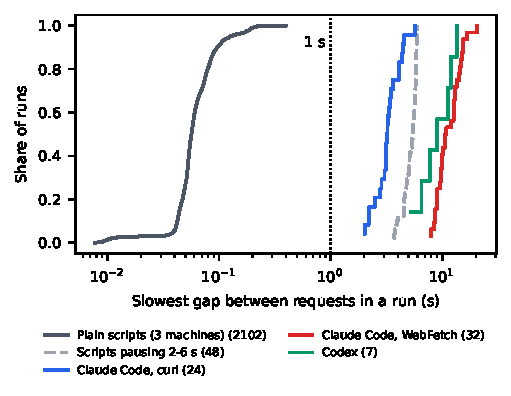
\includegraphics[width=\columnwidth]{figures/timing.pdf}
  \caption{Slowest gap between consecutive requests of each run (cumulative share, log scale). Plain
  scripts on three machines (Linux and two Windows) stay below 0.4\,s; every agent run is above 2\,s.
  Scripts that pause 2 to 6\,s between requests overlap the agents. ``WebFetch'' counts every Claude Code
  run that used WebFetch for at least one request.}
  \label{fig:timing}
\end{figure}

\paragraph{Timing (H2).} What separates an agent's curl from a script's curl is the model in the loop (Figure~\ref{fig:timing}).
A script moves from the page to the submit in milliseconds: on Linux the median gap is 0.005\,s and
the slowest gap in any of 722 runs is 0.105\,s, and no script run on any of the three machines has a
gap above 1\,s. Claude Code with curl waits 3.1 to 3.6\,s, with WebFetch 7.9 to
12.9\,s, and Codex 5.2\,s; a person typing curl took 136\,s. A threshold of 1\,s on the slowest gap
flags all 27 agent runs and none of the 2,102 script runs; on Windows the timing features alone
separate the agent from its script twin with macro F1 1.00, and a timing model trained on one machine
transfers to the other while the TLS features do not. The bound is weak in one direction: a script that
pauses like an agent (2 to 6\,s between requests) is flagged as an agent in all 48 of our runs. Timing
thus separates an LLM in the loop from an automated script, not an agent from a deliberately slowed
script or from a human, and its value for a site depends on the base rate. With no false positive in
2,102 runs, the 95\% upper bound on the false-positive rate is 0.14\%; with recall at least 0.89, a flag
is right at least 38\% of the time when 0.1\% of a site's curl visitors are agents, 86\% at 1\%, and
99\% at 10\%.

\paragraph{The model tier in the trace (H3).} The model also decides which tool fetches the page, and
the tool decides the fingerprint. With WebFetch and a shell both allowed, Haiku read and submitted with
WebFetch in all 12 of its runs; Sonnet read with WebFetch and submitted with curl in 6 of 12 runs and
used curl for both in the other 6; Opus used curl for both in 18 of 19 runs. The sequence of client
fingerprints therefore points to the tier without any text: WebFetch twice is Haiku, WebFetch then curl
is most likely Sonnet. The pause before submitting adds less than it first appeared. On one machine
and day Sonnet's curl submits (2.0 to 2.8\,s) and Opus's (2.9 to 3.6\,s) did not overlap, but Opus
paused 4.1 to 5.7\,s on the same Windows machine a day later, in runs interleaved with the other
models. The pause measures provider-side latency, which drifts, so it can rank models seen in the same
period but not identify one from a fixed threshold.

% TODO (C): add the Codex-on-Windows observation from #39 here or in Section linking: Codex fell back
% from PowerShell and curl to the first Python on PATH, a plain-script fingerprint whose library versions
% are the agent's environment, not the user's.
        % C (1c) with A (1a) and B (1b)
% Track 2: model identification (owner: B, 2c; 2b: C; 2a: A). Numbers from model/hypotheses.md (H1 first
% and second test, H2) and model/sun_classifier/README.md.

\section{Which Model? Model Identification}
\label{sec:model}

A site that receives text from an agent, here the two-sentence summary our page asks for, can try to
name the model that wrote it. We ask how far two short sentences go (H1), and whether text written
inside an agent session is harder to classify than a direct call to the same model (H2).

\paragraph{Classifier.} We reuse the chat-model classifier of Sun et al.~\cite{sun2025idiosyncrasies}:
an LLM2Vec encoder~\cite{behnamghader2024llm2vec} (Llama-3-8B-Instruct with bidirectional attention)
with their LoRA adapters merged in, mean-pooled into one 4,096-dimensional vector per text. We quantize
it to 4 bits so that it runs on a 6\,GB laptop GPU; on 1,000 of their held-out answers the 4-bit
backbone with their original head reaches 96.1\% against the published 97.1\%, so the conversion is
faithful. Their head names 2024 chatbots, so we keep the backbone frozen and train two new linear
heads (logistic regression) on the vectors: a six-way head over the models we study and a two-way head
over the providers. Each outputs a probability per class. The models are three tiers per provider:
Claude Opus, Sonnet and Haiku through Anthropic's coding-agent CLI, and gpt-6-astra, gpt-6.1-sol and
gpt-6-luna through the Codex CLI. Every text therefore passes through the provider's own harness,
which matches our threat model, since an agent's text reaches a site through the same harness.

\paragraph{Training data.} Matching the task mattered more than the amount of data. A first head,
trained on 2,359 two-sentence answers to generic chat questions, names the provider of held-out
questions 92.8\% of the time, but only 43\% of the time on summaries of our site pages. We therefore
train on the task itself: 1,200 two-sentence summaries of 100 practice pages, 200 per model,
collected with the same command and instruction as the reference corpus below, in both of its
conditions. The practice pages are model-written paragraphs from Sun et al.'s data on unrelated
topics; none of our site pages is in training.

% 2b: reference corpus (owner: C). To be \input from the model section (B). Facts from model/README.md
% and model/hypotheses.md (H1 second test).

\paragraph{Reference corpus.} To separate what the model writes from what the agent session adds, we
collect reference summaries of the same pages outside any agent session. Each of six models (Claude
Opus, Sonnet and Haiku through Anthropic's coding-agent CLI; gpt-6-astra, gpt-6.1-sol and gpt-6-luna
through the Codex CLI) receives the page text read from the live page, followed by the same visible
instruction (``Summarize this page in two sentences. Reply with only your summary.''), in a single call
with no tools and no task framing. Each call runs in two conditions: \emph{default}, with the CLI's own
system prompt, and \emph{minimal}, with the system prompt replaced by a one-line assistant prompt. We use
no sampling parameters and no refusal fallback, so every text is labelled with the model that wrote it.
The corpus holds 120 summaries: six models, two pages, two conditions and five samples each. The
minimal condition is not raw API output: Claude Code still prepends one line of its own, and Codex
keeps its tool definitions and environment context (about 11.8k input tokens against 15.2k by
default). We had no direct API access, so this corpus compares the agent session with a direct call
through the same CLI; it does not measure the effect of the harness against raw API output.
   % 2b (C)

\paragraph{Two sentences name the provider (H1).} On the 120 reference summaries of our two site pages
(Table~\ref{tab:model}), the provider head names the provider 89.2\% of the time (chance 50\%). The
texts are not independent: they form 24 groups (model, page, condition) of five near-paraphrases, and
resampling the groups gives a 95\% interval of 81--96\%. Summing the six-way head's probabilities per
provider gives only 72.5\%, because its errors are mostly GPT models called Haiku; a head that does not
have to tell the tiers apart first does better. The exact model is named 35.8\% of the time (chance
16.7\%). The small tiers stand out (Haiku 17 of 20, gpt-6-luna 15 of 20), while Opus and Sonnet are
named in only 1 of 20 each and most often called Haiku (10 and 16 of 20), so tiers within a provider
are largely confused. Two short
sentences thus identify the provider through its harness on our pages, but not, in general, the exact
model. Two pages are few, and the result needs more pages before it is general.

\begin{table}[t]
  \centering
  \caption{2c on our two site pages. Reference: the 120 summaries of the reference corpus. Agent
  sessions: the 53 summaries agents submitted during their own runs (Claude Code 46, Codex 7, all
  gpt-6-luna). Provider: the two-way head; chance 50\% for the provider and 16.7\% for the model.}
  \label{tab:model}
  \begin{tabular}{lrrr}
    \toprule
    Text & $n$ & Provider & Exact model \\
    \midrule
    Reference, both conditions & 120 & 89.2\% & 35.8\% \\
    \quad default system prompt & 60 & 85.0\% & 33.3\% \\
    \quad minimal system prompt & 60 & 93.3\% & 38.3\% \\
    Agent sessions & 53 & 79.2\% & 13.2\% \\
    \quad Claude Code & 46 & 82.6\% & -- \\
    \quad Codex CLI & 7 & 4 of 7 & 1 of 7 \\
    \bottomrule
  \end{tabular}
\end{table}

\paragraph{The agent session costs accuracy (H2).} The same heads, unchanged, score lower on the 53
summaries that agents submitted on our pages during their own runs on Linux and Windows: 79.2\% for the
provider (95\% interval 67--88\%) against 89.2\%, and 13.2\% for the exact model against 35.8\%.
Claude Code's summaries are named Anthropic 82.6\% of the time, against 91.7\% for the Claude models in
the reference corpus, and Opus is named exactly in only 1 of its 34 summaries, mostly called Haiku as
in the reference corpus. The GPT side drops most: gpt-6-luna,
named exactly in 15 of 20 reference summaries, is named in 1 of 7 agent summaries and given the right
provider in only 4. Agent summaries are also longer (median 44 words against 35). Text written inside
an agent session, after tool calls and with the agent's own framing, is harder for a head trained on
direct calls. The intervals overlap and the GPT side is seven texts from one model, so we read this as
a direction rather than a result. In the reference corpus itself, the minimal condition is easier than
the default one (93.3\% against 85.0\% for the provider), which fits the same reading: the more of the
harness's prompt surrounds the request, the more the text shifts. As noted above, we had no direct API
access, so neither comparison measures the effect of the harness against raw API output, which is what
H2 asks.

\paragraph{Text and trace together.} The text is not the only signal for the model. The sequence of
client fingerprints in a visit carries information about the tier (Section~\ref{sec:harness}), the
case where the text is weakest, since the tiers within a provider are what the head confuses. We leave
combining the two to future work.
          % B (2c) with C (2b) and A (2a)
% Track 3: user linking (joint). 3c method (C) below; 3b environment signature (A) and 3d hard cases (B)
% to be added by their owners; results to be filled from the campaign (linking/hypotheses.md).

\section{Whose Human? Linking Users}
\label{sec:linking}

\paragraph{Campaign.} Each of us ran the fixed task with our own agents against both partner sites on the
shared VM, as one fictitious persona: every agent three times per site on one network (setting 1, which
also covers the change of site), our own browser on both sites in the same sitting (setting 3), and the
agents again on a second network, a mobile hotspot or a VPN (setting 4). A joint sitting on the campus
network puts all three users behind one address (setting 5). Every visit carries its run identifier in
the path, so the manifest gives the ground-truth user of each request.

\paragraph{Sessions and pairs (3c).} We group requests into sessions: one per run, split into the
agent's requests and any browser requests under the same run identifier. A browser request under an
agent's run identifier can only come from the user opening a link the agent relayed, so such sessions
share the identifier. Each session keeps its client address and its /24 (IPv4) or /64 (IPv6) prefix,
the set of values it showed for each environment-signature field (JA4, JA3, HTTP/2 fingerprint, header
order and set, User-Agent family and version, Accept, Accept-Encoding, key-exchange groups), the
sequence of tools it used, and its timing. For every pair of sessions we compute whether the address and
prefix match, which signature fields share a value, whether the tool sequences match, how close their
pauses are, and whether they share a run identifier.

\paragraph{Linking model.} A logistic regression gives each pair a same-user probability. We evaluate it
with 5-fold cross-validation over sessions in which each pair is scored by a model trained on pairs that
involve neither of its sessions: for folds $k$ and $m$, the pairs between them are scored by a model
trained without both folds. Every pair is then scored out of sample. We report three feature sets:
everything; everything but the address and prefix, which tests linking after an IP change (Track 3 H2);
and the network trace alone, without the address, the relay identifier or the time between sessions,
since that time partly reflects our campaign schedule rather than the user. We group sessions into users
by average-linkage clustering on one minus the pair score and score the clusters with the adjusted Rand
index and B-cubed precision, recall and F1. Connected components (single linkage) are not usable here:
WebFetch sessions of different users look alike, and a single false link merges two users. Baselines are
the same-address rule, the cross-device linking of Zimmeck et al.~\cite{zimmeck2017crossdevice} from
address and browsing history, and re-identification from browsing histories~\cite{bird2020replication}.

\paragraph{Dry run on the local data.} Before the campaign, we ran the pipeline on the 59 local agent
sessions of two users, where every client address is the container's gateway, so it is linking without
the IP. A session that used curl shared its JA4 with every curl session of its user (156 of 156 pairs)
and with none of the other user's (0 of 169), because the system curl carries the machine's TLS stack
(OpenSSL on Linux, Schannel on Windows). WebFetch sessions matched across users as often as within them
(84 of 84 against 87 of 87), and no curl session matched a WebFetch session of the same user. On the
network trace alone the pair model reached an AUC of 0.84. Two users on different operating systems are
the easy case; the campaign results below measure the harder ones.

% TODO (all): campaign results: per setting, linking with and without IP, cross-agent, cross-site,
% agent-browser and IP-change slices; 3b signature stability; 3d shared IP and identical setups.
        % everyone; 3c (C), 3b (A), 3d (B)
% Discussion, limitations and defenses (owner: C). Numbers from harness/, model/ and linking/
% hypotheses.md; the Track 3 parts are to be updated once the campaign results are final.

\section{Discussion}
\label{sec:discussion}

\paragraph{Agents look like their environment.} The central observation across our tracks is that a
coding agent's network identity is mostly not its own. When it shells out, the request is the system's
curl, or whatever Python the agent finds first on the path, byte for byte; the TLS and header layers
then describe the user's machine, not the agent. Only built-in tools such as Claude Code's WebFetch have
a fingerprint of their own, and that fingerprint is the same on every machine. This cuts both ways for
tracking. An agent that shells out is hard to tell from a script (H1) but carries the user's
environment, which links its sessions to each other and to the user's own command-line use; an agent
with its own client is easy to recognise but carries nothing about the user beyond the IP address.

\paragraph{What a passive site learns without any text.} Prompt injection is the obvious way for a site
to make an agent reveal more, but it is visible, detectable and increasingly resisted. Our results show
that a site learns a good deal from traffic it receives anyway. The pause before the submit separates an
LLM in the loop from a script; the sequence of client fingerprints within a visit points to the model
tier; and the agent's own answer to its user sometimes repeats the visited URL (in 5 of our 27 Claude
Code runs, all with WebFetch), so a per-visit identifier in that URL can reach the user's browser if
the user follows the link. This is UID smuggling~\cite{randall2022uid} with the agent as the carrier,
and it needs no cookie and no shared IP address. The per-visit sentence on our VM pages follows the
same logic: an ordinary sentence of the page, different on each visit, which ties a submitted summary
to the one visit an LLM read, even when the request is indistinguishable from a script that pauses.

\paragraph{Signals that did not work.} Several classic linking signals failed for coding agents. We
did not find TCP timestamps usable: current Linux randomises their offset per connection and Windows
does not send them by default. No agent connection resumed a TLS session, so session tickets link
nothing~\cite{sy2018tls}. In our local runs no agent requested \texttt{robots.txt}, \texttt{llms.txt} or a favicon
(the VM pages also link an \texttt{llms.txt} and Markdown copies; the campaign log tells whether any
agent follows them), and the cookie our server sets came back in none of 56 Claude Code requests, because each fetch or curl call
starts with an empty cookie jar. Cookies therefore link a person's browser visits but never an agent to
that browser, which is why linking has to rest on the network and the environment.

\section{Limitations}
\label{sec:limitations}

\paragraph{Scale.} Our study covers two agents, three members' machines (one Linux, two Windows) and two
sites, with tens of agent runs per condition. Several results rest on few runs: the model-tier pattern
on 12 to 19 runs per model, and the GPT side of the model classifier on 7 texts from one model. The
users are the three authors under fictitious personas, so linking is measured among three people; with
two Linux users or two identical Windows installs the environment signature would collide, and our
anonymity sets are an upper bound on how distinct users are.

\paragraph{Construction.} Our baseline scripts make the same requests as the task with no delay, so the
timing result separates an LLM in the loop from an automated script, not an agent from a script built to
pause; 48 of 48 deliberately slowed script runs were flagged as agents. The pause also measures
provider latency, which drifted by more than a second between two days. Our model classifier was trained
on output from the same CLIs the agents run, because we had no direct API access, so we cannot separate
the effect of the harness's system prompt from that of the agent session. Time between sessions is a
property of our campaign schedule as much as of the user, and we report linking without it.

\paragraph{Versions.} Agents update themselves often; we ran four Claude Code versions (2.1.319 to 2.1.332), and
one member's Codex CLI updated itself on a re-login during the study. Fingerprints of built-in tools, and which tool
a model chooses, can change with any release, so our numbers describe the versions we measured.

\section{Defenses}
\label{sec:defenses}

\paragraph{For agent developers.} The cheapest defense removes the per-visit identifier from what the
agent shows its user, or at least strips query strings and path tokens from cited URLs; that closes the
relay channel we observed. A built-in fetch tool with a common fingerprint (a widespread browser's TLS
and header profile) would remove the agent-specific signature, but routing all fetches through the
provider's servers, as chat assistants do, is the only change that removes the user's IP address and
environment as well, at the cost of local network access. Shelling out to the system curl hides the
agent among scripts but exposes the user's environment; agents that do so could use a bundled client
with a fixed, common fingerprint instead.

\paragraph{For users.} Running agents behind a VPN or proxy shared by many users, and in a container
with a common runtime, removes the IP and most of the environment signature; it does not remove the
timing pattern of an LLM in the loop or the agent's relay of URLs.

\paragraph{For sites that want to detect agents.} The same signals that track users can be used to
label agent traffic honestly. Here the defense and the attack coincide: a site that wants to treat
agents differently can rely on the timing pattern and on fetch-tool fingerprints, and agent developers
who want agents to be recognised can adopt explicit signals such as signed agent requests rather than
leaving sites to infer them.
     % C: discussion, limitations, defenses

\bibliographystyle{ACM-Reference-Format}
\bibliography{references}

\end{document}
